\begin{figure}[!h]
    \centering
    \hspace{-1,5cm}
    \begin{subfigure}[b]{0.46\textwidth}
        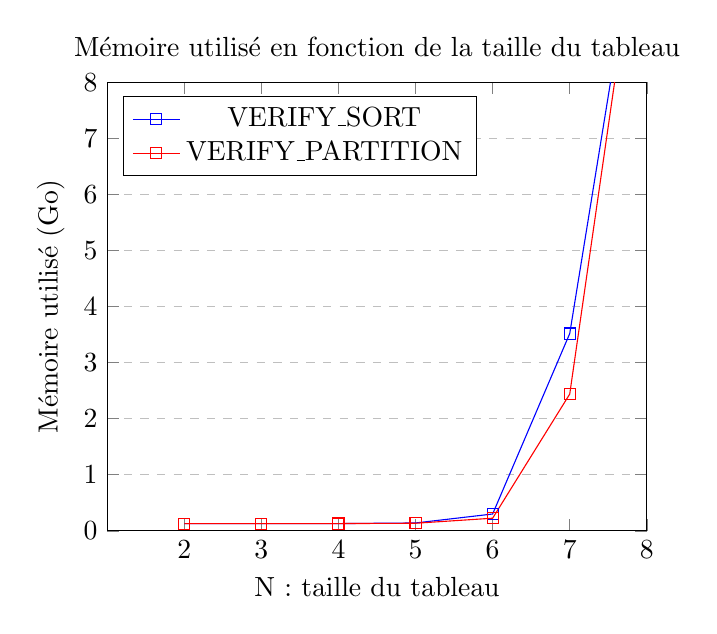
\begin{tikzpicture}%[scale=0.9]
        \begin{axis}[
            title={Mémoire utilisé en fonction de la taille du tableau},
            xlabel={N : taille du tableau},
            ylabel={Mémoire utilisé (Go)},
            xmin=1, xmax=8,
            ymin=0, ymax=8,
            xtick={2,3,4,5,6,7,8},
            ytick={0,1,2,3,4,5,6,7,8},
            legend pos=north west,
            ymajorgrids=true,
            grid style=dashed,
        ]

        \addplot[
            color=blue,
            mark=square,
            ]
            coordinates { % (x,y)(x,y)...
                (2,0.128)(3,0.128)(4,0.129)(5,0.140)(6,0.3)(7,3.52)(8,12)
            };
            \addlegendentry{VERIFY\_SORT}
         
        \addplot[
            color=red,
            mark=square,
            ]
            coordinates {
                (2,0.128)(3,0.128)(4,0.129)(5,0.135)(6,0.225)(7,2.44)(8,12)
            };
            \addlegendentry{VERIFY\_PARTITION}
        \end{axis}
        \end{tikzpicture}
    \end{subfigure}
    \hfill
    \begin{subfigure}[b]{0.46\textwidth}
        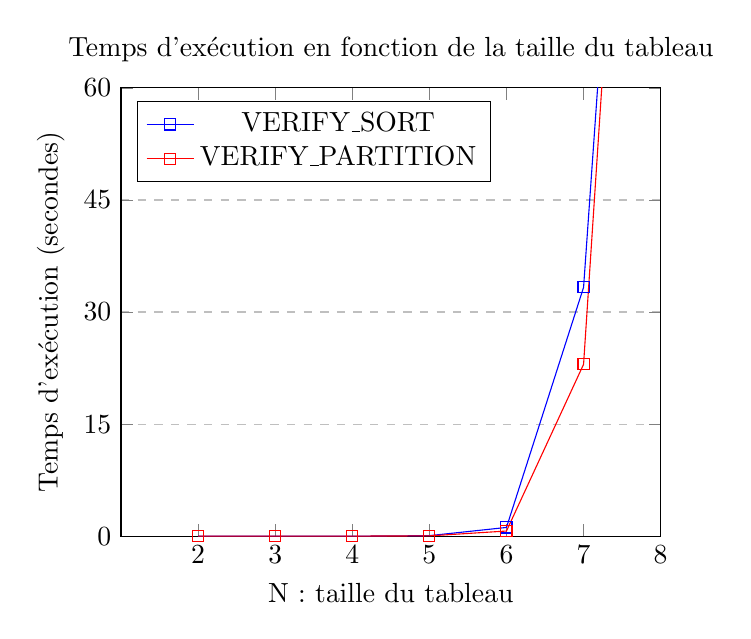
\begin{tikzpicture}%[scale=0.9]
        \begin{axis}[
            title={Temps d'exécution en fonction de la taille du tableau},
            xlabel={N : taille du tableau},
            ylabel={Temps d'exécution (secondes)},
            xmin=1, xmax=8,
            ymin=0, ymax=60,
            xtick={2,3,4,5,6,7,8},
            ytick={0,15,30,45,60},
            legend pos=north west,
            ymajorgrids=true,
            grid style=dashed,
        ]

        \addplot[
            color=blue,
            mark=square,
            ]
            coordinates {
                (2,0)(3,0)(4,0)(5,0.07)(6,1.17)(7,33.3)(8,180)
            };
            \addlegendentry{VERIFY\_SORT}
         
        \addplot[
            color=red,
            mark=square,
            ]
            coordinates {
                (2,0)(3,0)(4,0.01)(5,0.04)(6,0.69)(7,23)(8,180)
            };
            \addlegendentry{VERIFY\_PARTITION}
        \end{axis}
        \end{tikzpicture}
    \end{subfigure}
\end{figure}
